\subsection{Snailshell parametric equation}

\begin{table}[ht]
	\begin{center}
		\begin{tabular}[top]{ |p{16.0 cm}| }
			\rowcolor{LIGHTCYAN}			
			%% \hline \multicolumn{1}{|c|}{\textbf{Part 4/5 Snailshell and SnaHyp parametric curves}} \\ [1.0ex]
 

%% double scaleup = 100.0;
%% double k = (3.0*PI_cpos);
%% double x = ( sin(2*k*u) / (k*u*k*u + 4.0) );
%% return (scaleup)*(x);

%% double scaleup = 100.0;
%% double k = (3.0*PI_cpos);
%% double y = (cos(2*k*u) / (k*u*k*u + 4.0));
%% return (scaleup)*(y);
			
			\hline \textbf{No. 7 - Snailshell parametric curve}\\
			\begin{eqnarray}
				x(u) & = & 100\sin(6\pi u) / [9 (\pi u)^2 + 4] \nonumber \\   
				y(u) & = & 100\cos(6\pi u) / [9 (\pi u)^2 + 4] \nonumber \\
				u & \in & [0.0, 1.0] \nonumber
			\end{eqnarray}
			
			Open ended curve\\
			Overall No loop, smooth and continuous convex curves\\
			Reflection x-axis: non-symmetrical\\
			Reflection y-axis: non-symmetrical\\
			\frame{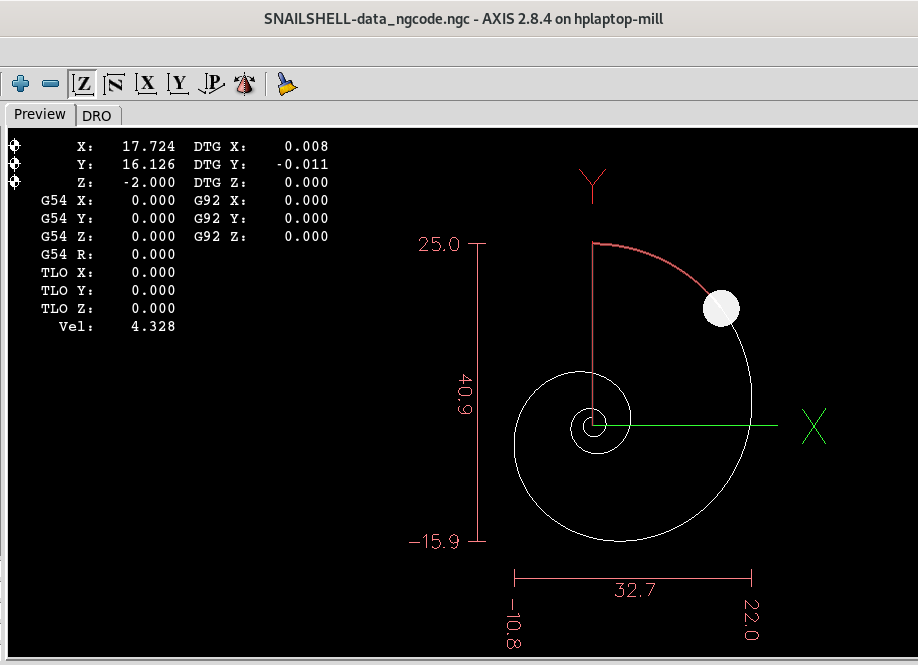
\includegraphics[width=0.550\textwidth]{./07-images/img-Ch5/SNAILSHELL-Axis.png}}
			\frame{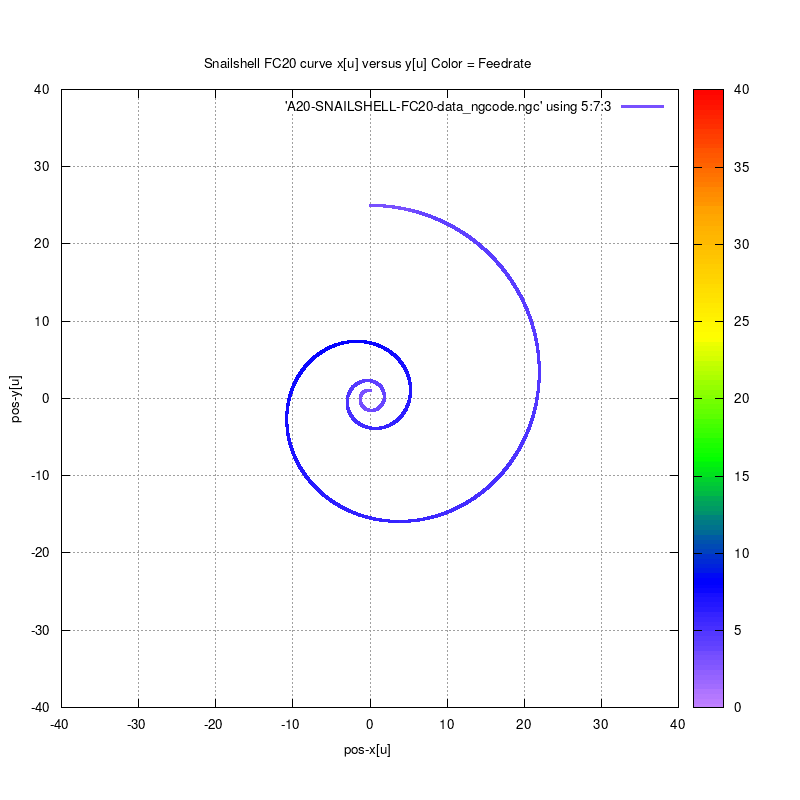
\includegraphics[width=0.395\textwidth]{./07-images/img-Ch5/SNAILSHELL-Feedrate.png}}\\
		
			\hline
		\end{tabular}
		\caption{Snailshell equation and dimensions}		
		\label{table:Snailshell equation and dimensions}
	\end{center}
\end{table}  
